\documentclass{article}
\usepackage{times}
\usepackage[english,russian]{babel}
\usepackage[utf8]{inputenc}
\usepackage{dirtytalk}
\usepackage[a4paper, total={6in, 8in}]{geometry}
\usepackage{graphicx}
\usepackage{hyperref}


\graphicspath{ {./img/} }

\begin{document}
\title{Лабораторная работа 1}

\date{\today}
\maketitle

\say{Сначала учите науку программирования и всю теорию. Далее выработаете свой программистский стиль. Затем забудьте все и просто программируйте.
— George Carrette}

\section{Введение}

Цель: изучить работу Ethereum, язык программирования Solidity


Для выполнения лабораторной работы, необходимо восопльзоватся виртуальной машиной, на которой установлена Ubuntu 18.04 и весь необходимый набор ПО.

Теорию можно прочесть в файле Theory.pdf.

(Тут будет инфа о пути к тестовому проекту)


\section{Подготовка окружения}

Все необходимые зависимости уже установлены на виртуальную машину. Далее будут представлены необходимые программы и пакеты для выполнения лабораторной работы. 

\subsection{Ganache}

Ganache - это блокчейн для разработки Ethereum, которую вы можете использовать для развертывания контрактов, разработки приложений и запуска тестов. Он создает виртуальную цепочку Ethereum и генерирует некоторые поддельные учетные записи, которые мы будем использовать во время разработки (Рис. 1).

Для запуска Ganache, найдите значек в меню приложений. Сразу после запука будут установлены значения по умолчанию, контролирующие количество поддельных учетных записей и сумму ETH на их счетах.

\begin{figure}
    \centering
    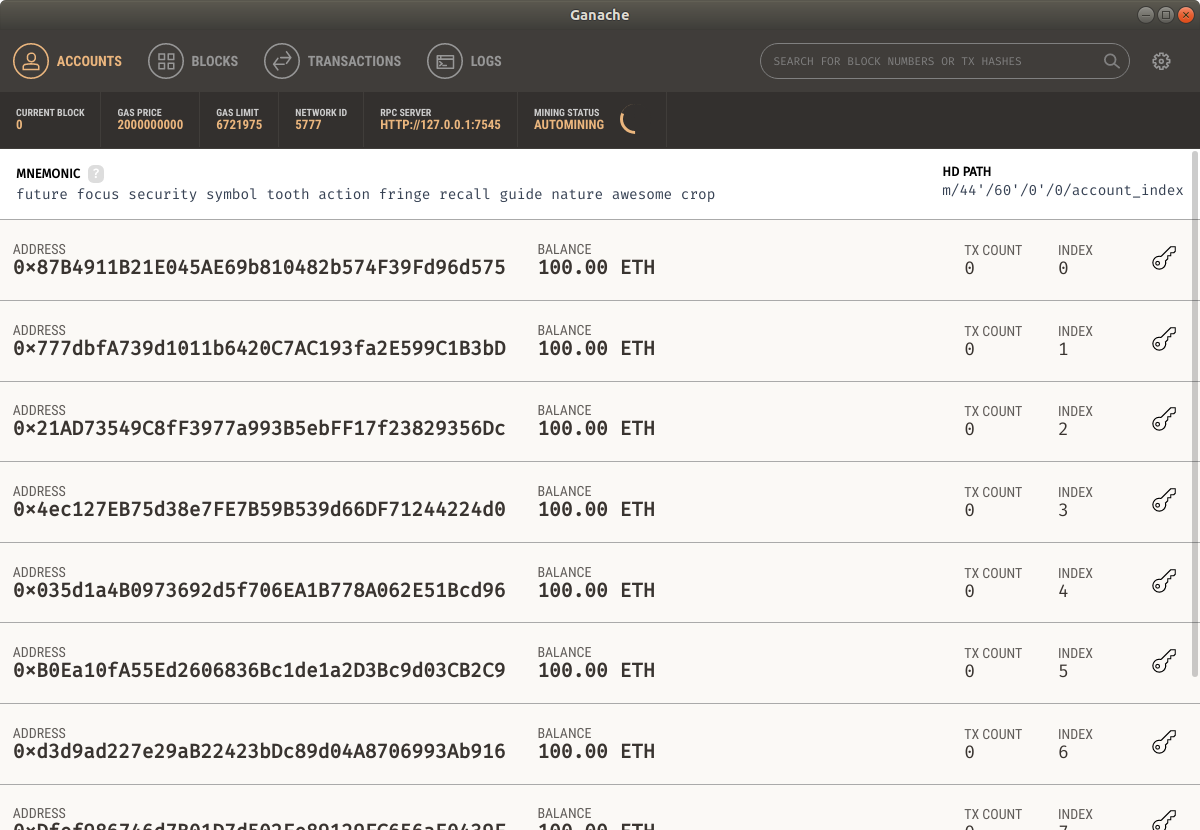
\includegraphics[scale=0.4]{ganache_1}
    \caption{Интерфейс Ganache.}
    \label{fig:ganache_1}
\end{figure}

\subsection{Metamask}

Metamask -  это криптовалютный кошелек, который встраивается в браузер Google Chrome и он нужен для упрощения передачи Эфира (Эфириум,  Ethereum, ETH)  или токенов ERC-20  в сети Эфириума. Мы будем использовать его для тестирования смарт-контрактов.


\begin{figure}
    \centering
    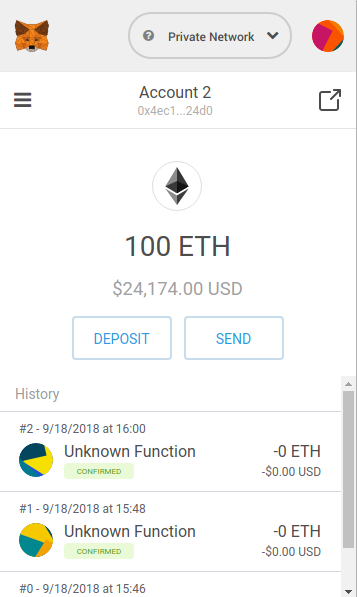
\includegraphics[scale=0.4]{metamask_1}
    \caption{Интерфейс MetaMask.}
    \label{fig:metamask_1}
\end{figure}

\subsection{Metamask}



\begin{thebibliography}{9}

	\bibitem{lamport94}
	  \emph{Как работает Эфириум (Ethereum)?}
	  https://habr.com/post/407583/

\end{thebibliography}

\end{document}